\textbf{Implementación del molino de carne }

Para realizar la operación del triturado del sistema, se determinó utilizar un molino de carne. Para implementarlo, fue necesario lavar el dispositivo para retirarle la cubierta de estaño que traía de fábrica, ya que esta capa se suele caer por sí sola a lo largo del tiempo, pero puede ser perjudicial para la generación del compost.

Una vez lavado, fue necesario realizarle un rectificado a las patas del triturador con ayuda de un esmeril. De esta manera, se aseguró de que se tenga una mayor superficie de contacto y, por ende, evitar vibraciones al momento de ser atornillado a la estructura.

También se colocó una polea de 14 pulgadas de diámetro a la entrada del eje, para recibir el impulso que haga rotar al tornillo sin fin por medio de una banda.\\
\clearpage

\textbf{Implementación de la motorización del sistema de trituración.}

Esta parte se agregó al sistema con el fin de facilitarle al usuario la trituración de los residuos orgánicos, buscando que el sistema sea amigable con el usuario.

Para este fin, se utilizó un motor de corriente alterna que fue extraído de una lavadora de 16 kg. Al ser un motor muy potente que gira a una velocidad de 1450 rpm, se propuso utilizar un dimmer de 400 $W$ para disminuir su velocidad angular. Además de emplear un juego de poleas para obtener una velocidad de 207 rpm a la entrada del triturador.

El control de la velocidad en este caso es muy importante, debido a que, si el tornillo sin fin del triturador gira a la misma velocidad que el motor, puede provocar daños a todo el molino. Asimismo, la generación de vibraciones podría deformar la estructura o dañar componentes a largo plazo.

Este motor se activa de manera manual, gracias a una botonera que está en un costado de la estructura. Es así que el control de la trituración está en manos del usuario, por lo que no depende de los demás sistemas para funcionar y sigue siendo un sistema semiautomático que requiere de un operador para realizar algunas tareas.
 
A la salida del triturador, se colocó una tubería de PVC con la que se encaminan los desechos hacia el interior del contenedor para su procesamiento. Por lo que el sistema de entrada de la materia orgánica se aprecia en la figura. (\ref{fg:sist_tritura_fisico}).

\begin{figure}[h]
            \centering
            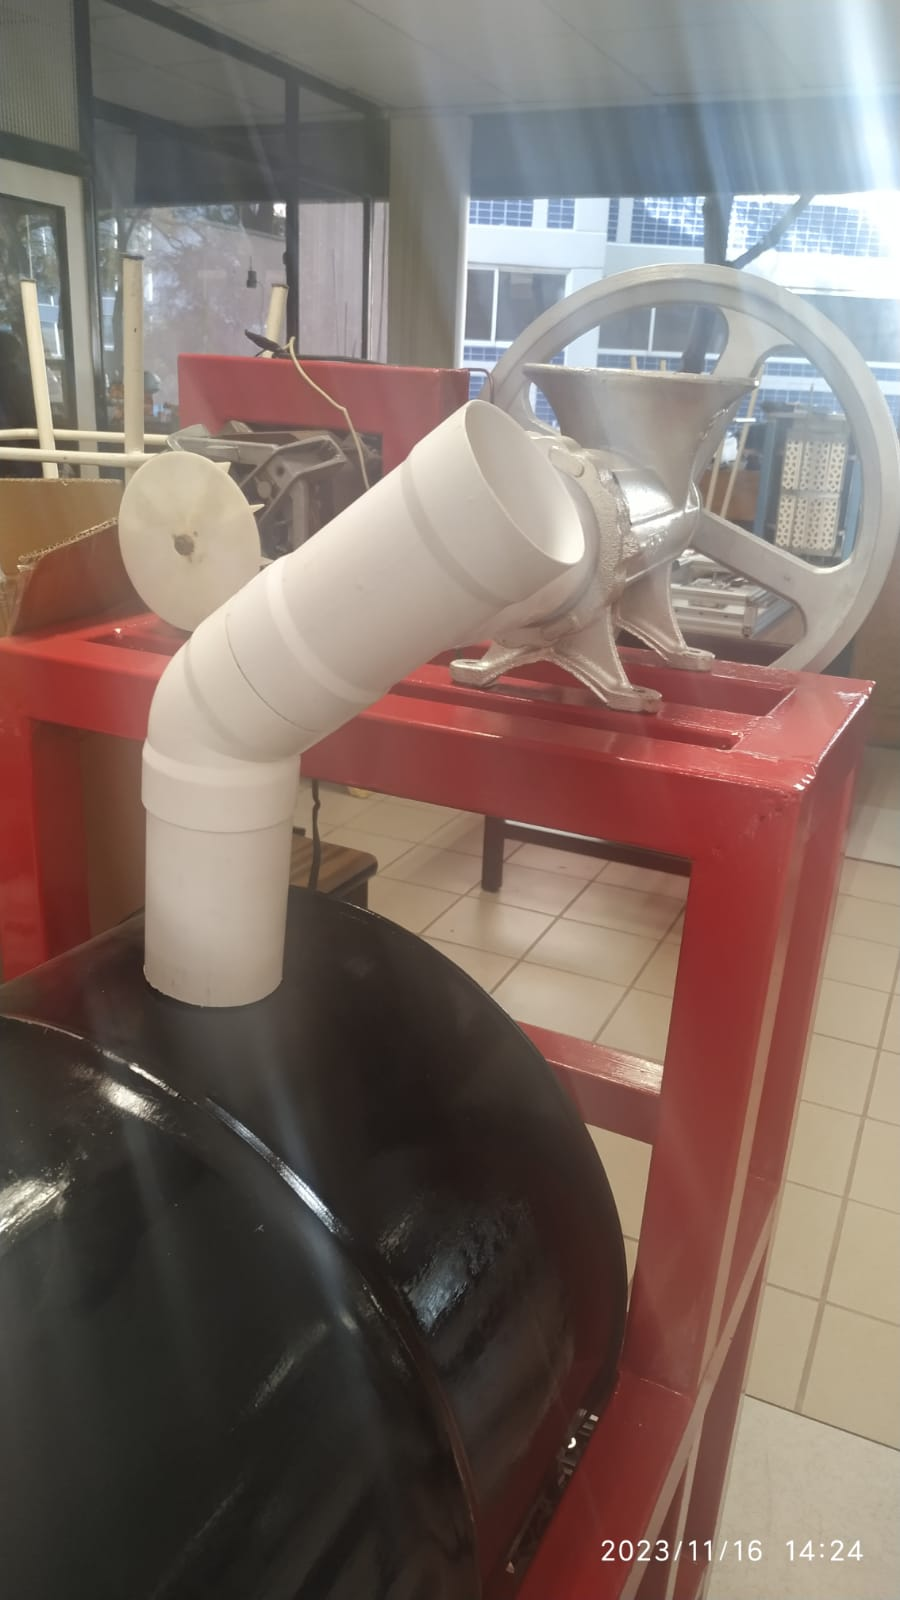
\includegraphics[scale=0.3]{images/Capitulo_Imple/S4/trituracion.jpeg}
            \caption{Sistema de trituración montado}
            \label{fg:sist_tritura_fisico}
\end{figure}

\clearpage